%%%%%%%%%%%%%%%%%%%%%%%%%%%%%%%%%%%%%%%%%%%%%%%%%%%%%%%%%%%%%%%%%%
\section{Flexible beam in a confined channel flow}
\label{sec:beamtunnel}
%%%%%%%%%%%%%%%%%%%%%%%%%%%%%%%%%%%%%%%%%%%%%%%%%%%%%%%%%%%%%%%%%%

The first coupled verification is the soft-beam case of \citet{zhang_immersed_2012} (Section~6.4, Case~1), in which a slender flexible cantilever clamped to the no-slip wall of a narrow channel is bent into a steady deformed shape by a steady, pressure-driven viscous flow. It is an established benchmark for immersed and meshless FSI formulations \citep{long_coupling_esfem_sph_2021,wang_immersed_esfem_2022,yang_peridynamics_iblbm_2022,yan_explicit_velocity_iblbm_2023}. Because the flow is steady and the cantilever settles into a fixed shape, the problem reduces to a static equilibrium in which the drag distributed along the deflected beam is balanced everywhere by the elastic restoring moment. That steadiness is what makes it a convenient first test, since there is no moving interface to capture, no time variation of the inflow, and no vortex shedding.

Every reference study resolves the cantilever as a two-dimensional continuum, and they differ from one another only in the fluid solver and the interface coupling, as Table~\ref{tab:beamtunnel_refstudies} shows. Here the square cross-section enters the formulation only through its area, its second moment of area, and the drag reference length of Section~\ref{sec:almLineForce}, and the domain is one cell thick in the third direction, so the simulation is effectively two-dimensional while the physical thickness of the beam is still carried by the projection operators. What the benchmark tests is therefore whether a one-dimensional beam loaded by a distributed normal drag can reproduce the deflection that a resolved two-dimensional continuum gives, in a confined flow at low Reynolds number. The outcome is not obvious in advance, because collapsing the cross-section onto a line discards the resolved pressure and viscous tractions on the beam faces and replaces them with a single drag coefficient. The reduction can be trusted only once the tip deflection it predicts falls within the spread of the fully resolved reference solutions.

\begin{table}[!ht]
\centering
\small
\caption{Published studies of the flexible-beam-in-channel benchmark of \citet{zhang_immersed_2012} (Section~6.4, Case~1).}
\label{tab:beamtunnel_refstudies}
\setlength{\tabcolsep}{5pt}
\renewcommand{\arraystretch}{1.30}
\begin{tabularx}{\linewidth}{l X X X}
\toprule
Study & Structural model & Fluid solver & Coupling \\
\midrule
\citet{zhang_immersed_2012}          & 2D ES-FEM-T3 continuum          & Characteristic Galerkin FEM            & Immersed smoothed FEM \\
\citet{long_coupling_esfem_sph_2021} & 2D ES-FEM continuum             & Smoothed particle hydrodynamics        & Fictitious boundary particles \\
\citet{yan_explicit_velocity_iblbm_2023} & 2D smoothed point interpolation & Hybrid lattice-Boltzmann flux solver & Immersed boundary \\
\citet{yang_peridynamics_iblbm_2022} & 2D bond-based peridynamics      & Lattice-Boltzmann                      & Multi-direct-forcing IB \\
\citet{wang_immersed_esfem_2022}     & 2D ES-FEM continuum             & Edge-based smoothed FEM fluid          & Immersed ES-FEM/ES-FEM \\
\midrule
Present work                          & 1D Simo--Reissner FV beam       & Finite volume Navier--Stokes (OpenFOAM) & Actuator-line distributed forcing \\
\bottomrule
\end{tabularx}
\end{table}

\subsection{Problem definition}
\label{sec:beamtunnel_geometry}
The geometry is presented in Figure~\ref{fig:beamInTunnel_schematic}. The fluid domain is a rectangular channel of streamwise length $L = 4\times10^{-2}~\mathrm{m}$ and transverse height $H = 1\times10^{-2}~\mathrm{m}$, with the origin where the inlet plane meets the lower no-slip wall, $x$ measured downstream and $y$ upward. A slender flexible cantilever of length $b = 8\times10^{-3}~\mathrm{m}$ and uniform square cross-section of side $a = 4\times10^{-4}~\mathrm{m}$ is clamped at $x = L/4$ on the lower wall and extends upward into the flow, occupying $80\%$ of the channel height when undeformed. The thickness-to-length ratio $a/b = 1/20$ places the beam in the slender-cantilever regime. All quantities are reported in SI units; the original reference reports them in centimetres and grams, which are converted without modification.

\begin{figure}[!ht]
\centering
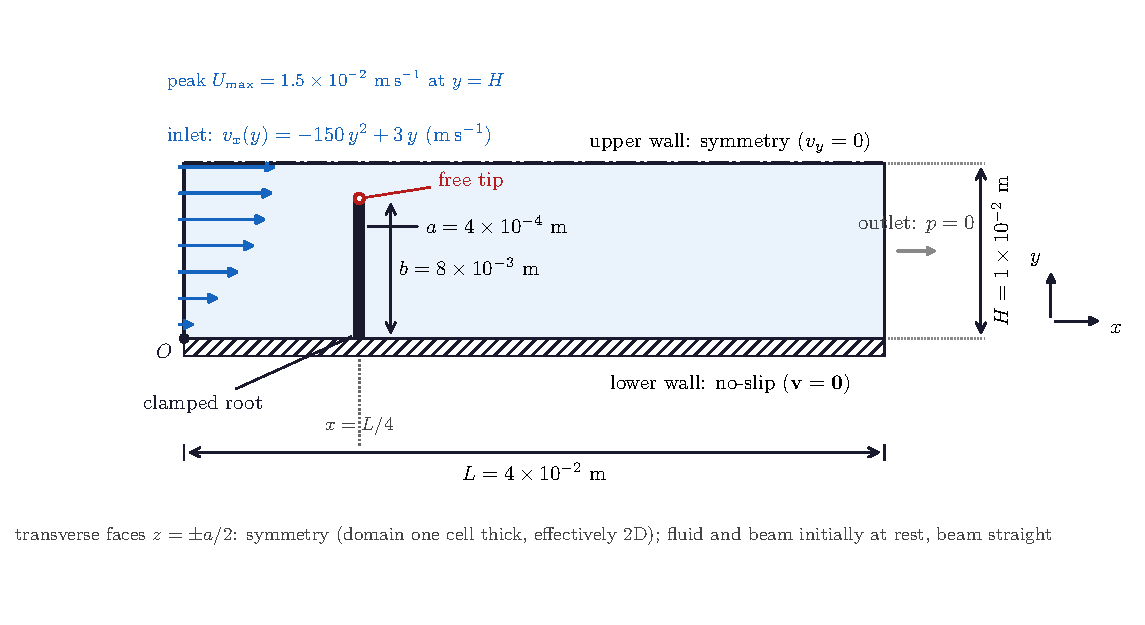
\includegraphics[width=0.95\textwidth]{beamInTunnel_schematic.pdf}
\caption{The flexible-beam-in-channel verification problem. The origin $O$ lies where the inlet plane meets the lower wall, with $x$ measured downstream and $y$ upward. The cantilever of length $b$ and square cross-section of side $a$ is clamped at $x = L/4$ on the lower no-slip wall and free at its tip. A steady parabolic profile is imposed at the inlet, a zero-pressure outflow on the right, the lower wall is no-slip, and the upper wall is a symmetry plane. Dimensions reproduce \citet{zhang_immersed_2012}, Section~6.4, Case~1, converted to SI units.}
\label{fig:beamInTunnel_schematic}
\end{figure}

A steady parabolic horizontal velocity profile is prescribed at the inlet,
\begin{equation}
v_x(y) = -150\,y^2 + 3\,y~~~\mathrm{m\,s^{-1}}, \qquad v_y(y) = 0,
\label{eq:beamtunnel_inlet}
\end{equation}
with $y$ in metres, which is the SI form of the profile $v_x = 1.5(-y^2 + 2y)~\mathrm{cm\,s^{-1}}$ reported in the original paper. It vanishes at the lower wall and attains $U_{\max} = 1.5\times10^{-2}~\mathrm{m\,s^{-1}}$ at the upper symmetry plane. The downstream boundary is a zero-gradient outflow with a fixed reference pressure, the lower boundary a stationary no-slip wall on which the cantilever root is clamped, and the upper boundary a symmetry plane, consistent with the half-domain interpretation of the reference paper in which the mirror across $y = H$ recovers an infinite array of identical cantilevers. The two transverse faces are also symmetry boundaries. Both the fluid and the beam start at rest, with the beam undeformed, and the simulation is advanced with $\Delta t = 10^{-4}~\mathrm{s}$ to $t = 2.5~\mathrm{s}$, by which point the tip velocity has vanished.

Properties are listed in Table~\ref{tab:beamtunnel_properties} and are taken without modification from the reference. The beam follows a linear elastic law with Young's modulus $E$ and Poisson ratio $\nu_s$, from which the shear modulus follows as $G = E/[2(1+\nu_s)]$, so the axial, shear, bending, and torsional responses are all governed by one linear elastic law. The reference uses a Saint-Venant--Kirchhoff hyperelastic continuum, but the deformations in Case~1 remain small in the strain sense because the cantilever bends as a slender beam rather than stretching, so the linear law used here produces an equivalent constitutive response in this regime. The flow regime is characterised by a thickness-based Reynolds number $\mathrm{Re}_a = \rho\,U_{\max}\,a/\mu \approx 0.6$, in the viscous-dominated Stokes-like regime, with a height-based value of $15$. Gravity is neglected, consistent with the reference.

\begin{table}[!ht]
\centering
\small
\caption{Fluid and beam properties for the flexible-beam-in-channel verification problem, following \citet{zhang_immersed_2012}, Section~6.4, Case~1.}
\label{tab:beamtunnel_properties}
\setlength{\tabcolsep}{6pt}
\renewcommand{\arraystretch}{1.15}
\begin{tabularx}{\linewidth}{l c X}
\toprule
Quantity & Symbol & Value \\
\midrule
\multicolumn{3}{l}{\textbf{Fluid domain}} \\
\cmidrule(lr){1-3}
Channel length (streamwise)      & $L$    & $4.0\times10^{-2}~\mathrm{m}$ \\
Channel height                   & $H$    & $1.0\times10^{-2}~\mathrm{m}$ \\
Fluid density                    & $\rho$ & $1.0\times10^{3}~\mathrm{kg\,m^{-3}}$ \\
Dynamic viscosity                & $\mu$  & $1.0\times10^{-2}~\mathrm{Pa\,s}$ \\
Peak inlet velocity              & $U_{\max}$ & $1.5\times10^{-2}~\mathrm{m\,s^{-1}}$ \\
\midrule
\multicolumn{3}{l}{\textbf{Beam}} \\
\cmidrule(lr){1-3}
Length                           & $b$        & $8.0\times10^{-3}~\mathrm{m}$ \\
Cross-section side               & $a$        & $4.0\times10^{-4}~\mathrm{m}$ \\
Solid density                    & $\rho_s$   & $7.8\times10^{3}~\mathrm{kg\,m^{-3}}$ \\
Young's modulus                  & $E$        & $1.0\times10^{4}~\mathrm{Pa}$ \\
Poisson ratio                    & $\nu_s$    & $0.3$ \\
\bottomrule
\end{tabularx}
\end{table}

\subsection{Steady-CFD calibration of the normal drag coefficient}
\label{sec:beamtunnel_cd_calibration}

The normal drag coefficient in Eq.~\eqref{eq:almLineForce} has to be fixed before the coupled result can be discussed. Because the formulation reduces the cross-section to a centreline, the near-field pressure and viscous tractions on the deformed cross-section are not resolved by the fluid solver, and are absorbed instead into a single effective coefficient multiplying the upstream-sampled velocity squared. Selecting a value that reflects the actual confined-channel drag on a rigid cross-section of the same geometry is therefore a prerequisite for trusting the coupled result.

A separate steady incompressible CFD simulation was run on the same channel domain, with the flexible cantilever replaced by an undeformed rigid plate of the same square cross-section clamped at the same root location. The geometry, boundary conditions, and fluid properties are identical to the coupled case, and the only difference is that the plate is held rigid. The case is solved with \texttt{simpleFoam} on a uniform $150 \times 38$ background hexahedral mesh with one level of local refinement around the plate (Figure~\ref{fig:beamInTunnel_dragcalib_mesh}), which captures the upstream stagnation point, the accelerated jet between the plate tip and the upper symmetry boundary, and the leeward recirculation. The reference area is $A_{\mathrm{ref}} = a b = 3.2\times10^{-6}~\mathrm{m^2}$, so the reported coefficient corresponds directly to the normal drag coefficient of the closure. The plate is held straight while the coupled beam bends downstream and blocks less of the channel at equilibrium, which matters less than it appears, because the actuator line multiplies $C_{dn}$ by the velocity it samples at each node in the deformed configuration, and that velocity already reflects the wider gap above the deflected tip.

\begin{figure}[!ht]
\centering
\begin{subfigure}[b]{0.55\textwidth}
  \centering
  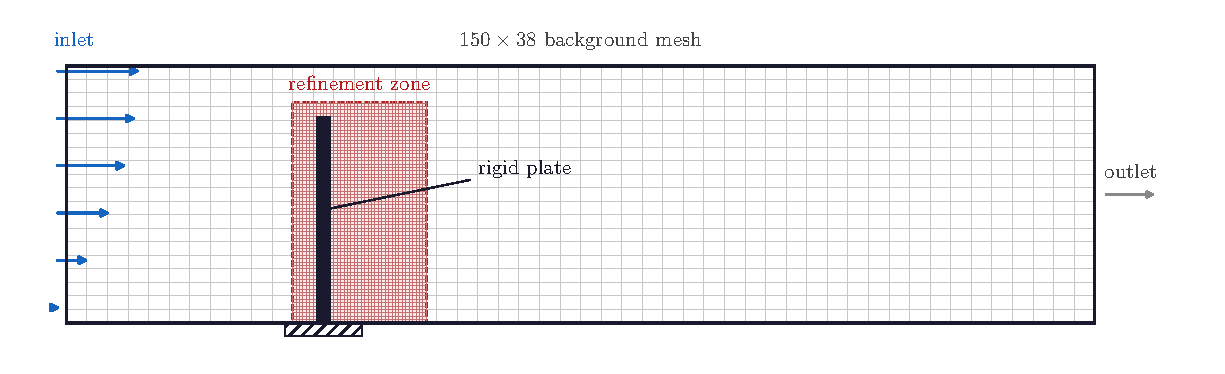
\includegraphics[width=\linewidth]{dragCalib_mesh_schematic.pdf}
  \caption{}
  \label{fig:beamInTunnel_dragcalib_mesh}
\end{subfigure}\hfill
\begin{subfigure}[b]{0.43\textwidth}
  \centering
  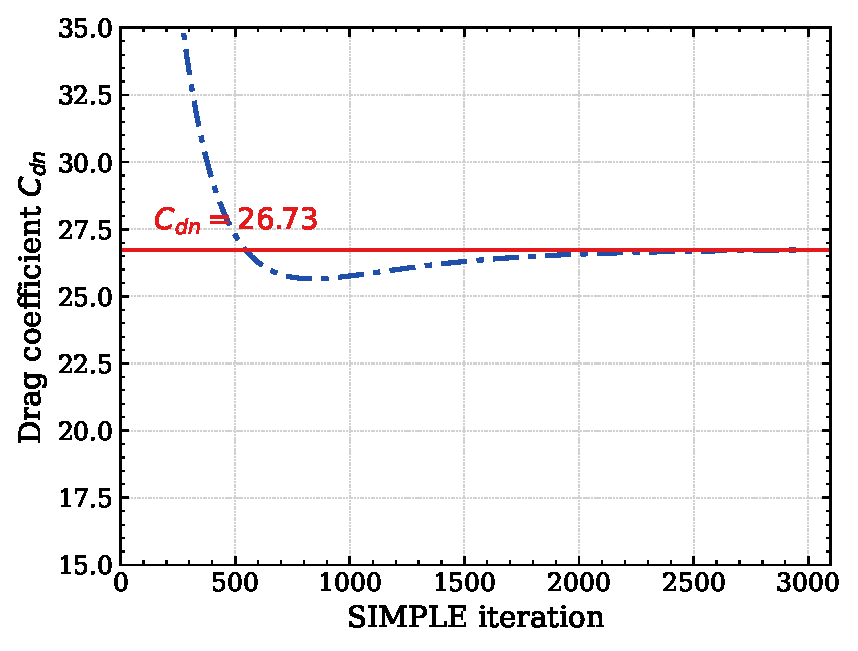
\includegraphics[width=\linewidth]{cd_calibration.pdf}
  \caption{}
  \label{fig:beamInTunnel_cd_calibration}
\end{subfigure}
\caption{Steady-CFD calibration of the normal drag coefficient. (a) Mesh topology: a uniform $150 \times 38$ background mesh with one level of local refinement around the rigid plate (red zone), which occupies the same root location and cross-section as the flexible cantilever. (b) Convergence of $C_{dn}$ over the SIMPLE outer iterations (blue dash-dotted), with the converged value $C_{dn} = 26.73$ marked in red.}
\label{fig:beamInTunnel_dragcalib}
\end{figure}

Figure~\ref{fig:beamInTunnel_cd_calibration} reports the convergence history. A rapid initial transient brings $C_{dn}$ down to approximately $25.5$ at iteration $700$, after which a slow drift, reflecting the residual pressure adjustment in the highly viscous flow, carries it toward an asymptotic value of $26.7$ at iteration $2950$, the change between iterations $2000$ and $2950$ being below $0.5\%$. The value $C_{dn} = 26.73$ is read directly off the converged plateau. No rounding or empirical adjustment is applied, and no further tuning against the reference tip displacement is performed in the coupled simulation, so the calibration is a single one-way handover from the rigid-plate CFD to the coupled run. The companion tangential coefficient is fixed at $C_{dt} = 0.01$, which represents skin friction along the beam faces rather than form drag on the cross-section, and a smooth surface at these Reynolds numbers has a friction coefficient of about this size, one to two orders of magnitude below the drag coefficient of a bluff cross-section \citep{hoerner_fluid_1965}. The geometry makes the value matter even less, because the beam stays close to normal to the flow and the tangential load contributes little to the bending.

This calibration is a one-time, geometry-specific step, not a free parameter of the method, and it is not a standing requirement of the coupling either. What makes it necessary here is confinement. The undeformed cantilever spans $80\%$ of the channel height, so the drag on it is set by the proximity of the walls as much as by the cross-section itself, whereas the generic correlations one might reach for instead, such as the flat-plate values of \citet{hoerner_fluid_1965} or the low-Reynolds cylinder estimate from Oseen's linearisation \citep{lamb_hydrodynamics_1932}, are derived for a body in an unbounded stream. Reading $C_{dn}$ off a steady CFD run on the confined geometry sidesteps that mismatch, and the same procedure can be repeated for any new blockage ratio. In an unbounded or weakly confined flow no such run is needed, and the wave-driven stem of Section~\ref{sec:flexveg} is handled in exactly that way, with the coefficient taken from drag fits published alongside the reference experiment. Confinement does not change the form of the closure, which remains a quadratic drag law acting normal to the centreline. What it changes is the value of the coefficient, and the source that value has to come from.

\subsection{Verification against the reference solutions}
\label{sec:beamtunnel_verification}

With $C_{dn}$ fixed, the coupled simulation is run to steady state. Figure~\ref{fig:beamInTunnel_verification} compares the predicted steady tip horizontal displacement against the range reported in the literature. The shaded reference range spans $4.7$ to $6.0~\mathrm{mm}$ and brackets the steady tip displacements digitised from the published curves of \citet{zhang_immersed_2012}, \citet{long_coupling_esfem_sph_2021}, and \citet{yan_explicit_velocity_iblbm_2023}. Two further references, \citet{yang_peridynamics_iblbm_2022} and \citet{wang_immersed_esfem_2022}, report values below this band; they are noted for completeness but excluded from it, being outliers relative to the original result and the more recent values from other methods.

\begin{figure}[!ht]
\centering
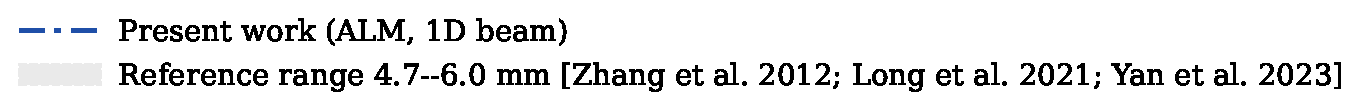
\includegraphics[width=0.90\textwidth]{verificationLegend.pdf}\\[0.4em]
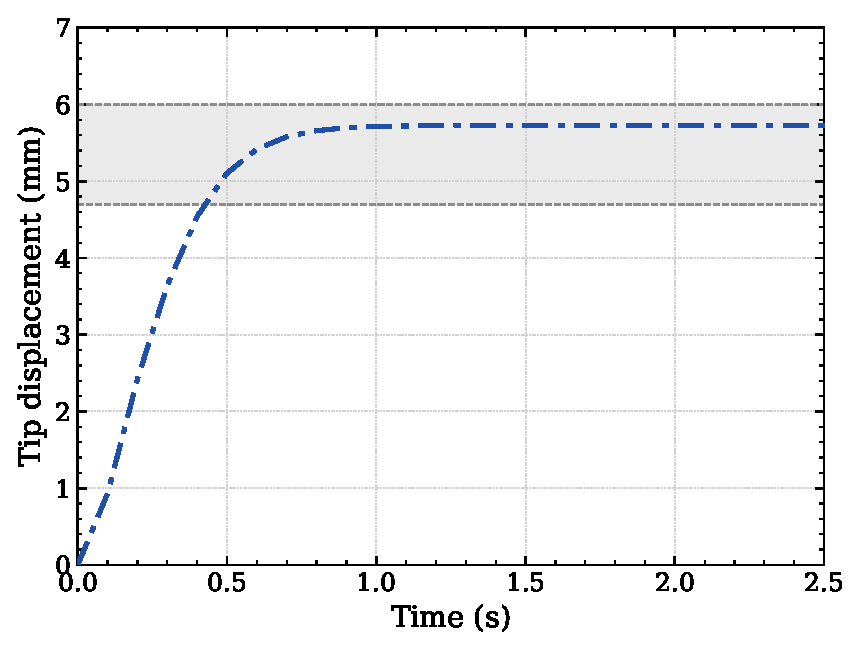
\includegraphics[width=0.68\textwidth]{verification.pdf}
\caption{Steady tip horizontal displacement of the flexible cantilever in the channel benchmark. The blue dash-dotted curve is the present result; the grey band spans the range $4.7$ to $6.0~\mathrm{mm}$ covered by the three closely clustered reference studies \citep{zhang_immersed_2012,long_coupling_esfem_sph_2021,yan_explicit_velocity_iblbm_2023}. The two outlier references \citep{yang_peridynamics_iblbm_2022,wang_immersed_esfem_2022} lie below the band and are listed in the legend for completeness.}
\label{fig:beamInTunnel_verification}
\end{figure}

The present transient reaches a stationary plateau at approximately $t = 1.4~\mathrm{s}$, and the converged tip displacement is $5.73~\mathrm{mm}$, inside the reference band. The two are not expected to converge to the same answer under mesh refinement, because the reference methods resolve the solid and the tractions on its faces while the present formulation replaces them with a drag law on a line, so the underlying mathematical models differ. Where the present value sits within the band follows from that idealisation. Even with $C_{dn}$ fixed at the rigid-plate value, the bent cross-section can develop a small additional pressure asymmetry that the rigid-plate calibration does not see. There is also no single agreed value within the family of two-dimensional continuum methods, and the width of the consensus band together with the spread of the outliers reflects sensitivities to the structural discretisation, the smoothing kernel adopted in the immersed coupling, and the treatment of the singular pressure field at the sharp upstream corners of the beam.

Figure~\ref{fig:beamInTunnel_snapshots} shows the flow field early in the transient and at the steady asymptote. At $t = 0.3~\mathrm{s}$ the tip has swung downstream by roughly half of its final displacement and the streamlines bend smoothly around the bent cantilever, but no closed recirculation cell has yet formed in the leeward region. The cell emerges between $t = 0.3$ and $0.6~\mathrm{s}$ together with an accelerated jet above the tip, and by $t = 1.5~\mathrm{s}$ the field is indistinguishable from its steady asymptote. The jet reaches $2.9\times 10^{-2}~\mathrm{m\,s^{-1}}$, almost twice the inlet peak velocity, the leeward eddy is fully developed, and the streamlines downstream relax back towards a quasi-parabolic profile by the outlet.

\begin{figure}[!ht]
\centering
\begin{subfigure}[b]{0.90\textwidth}
  \centering
  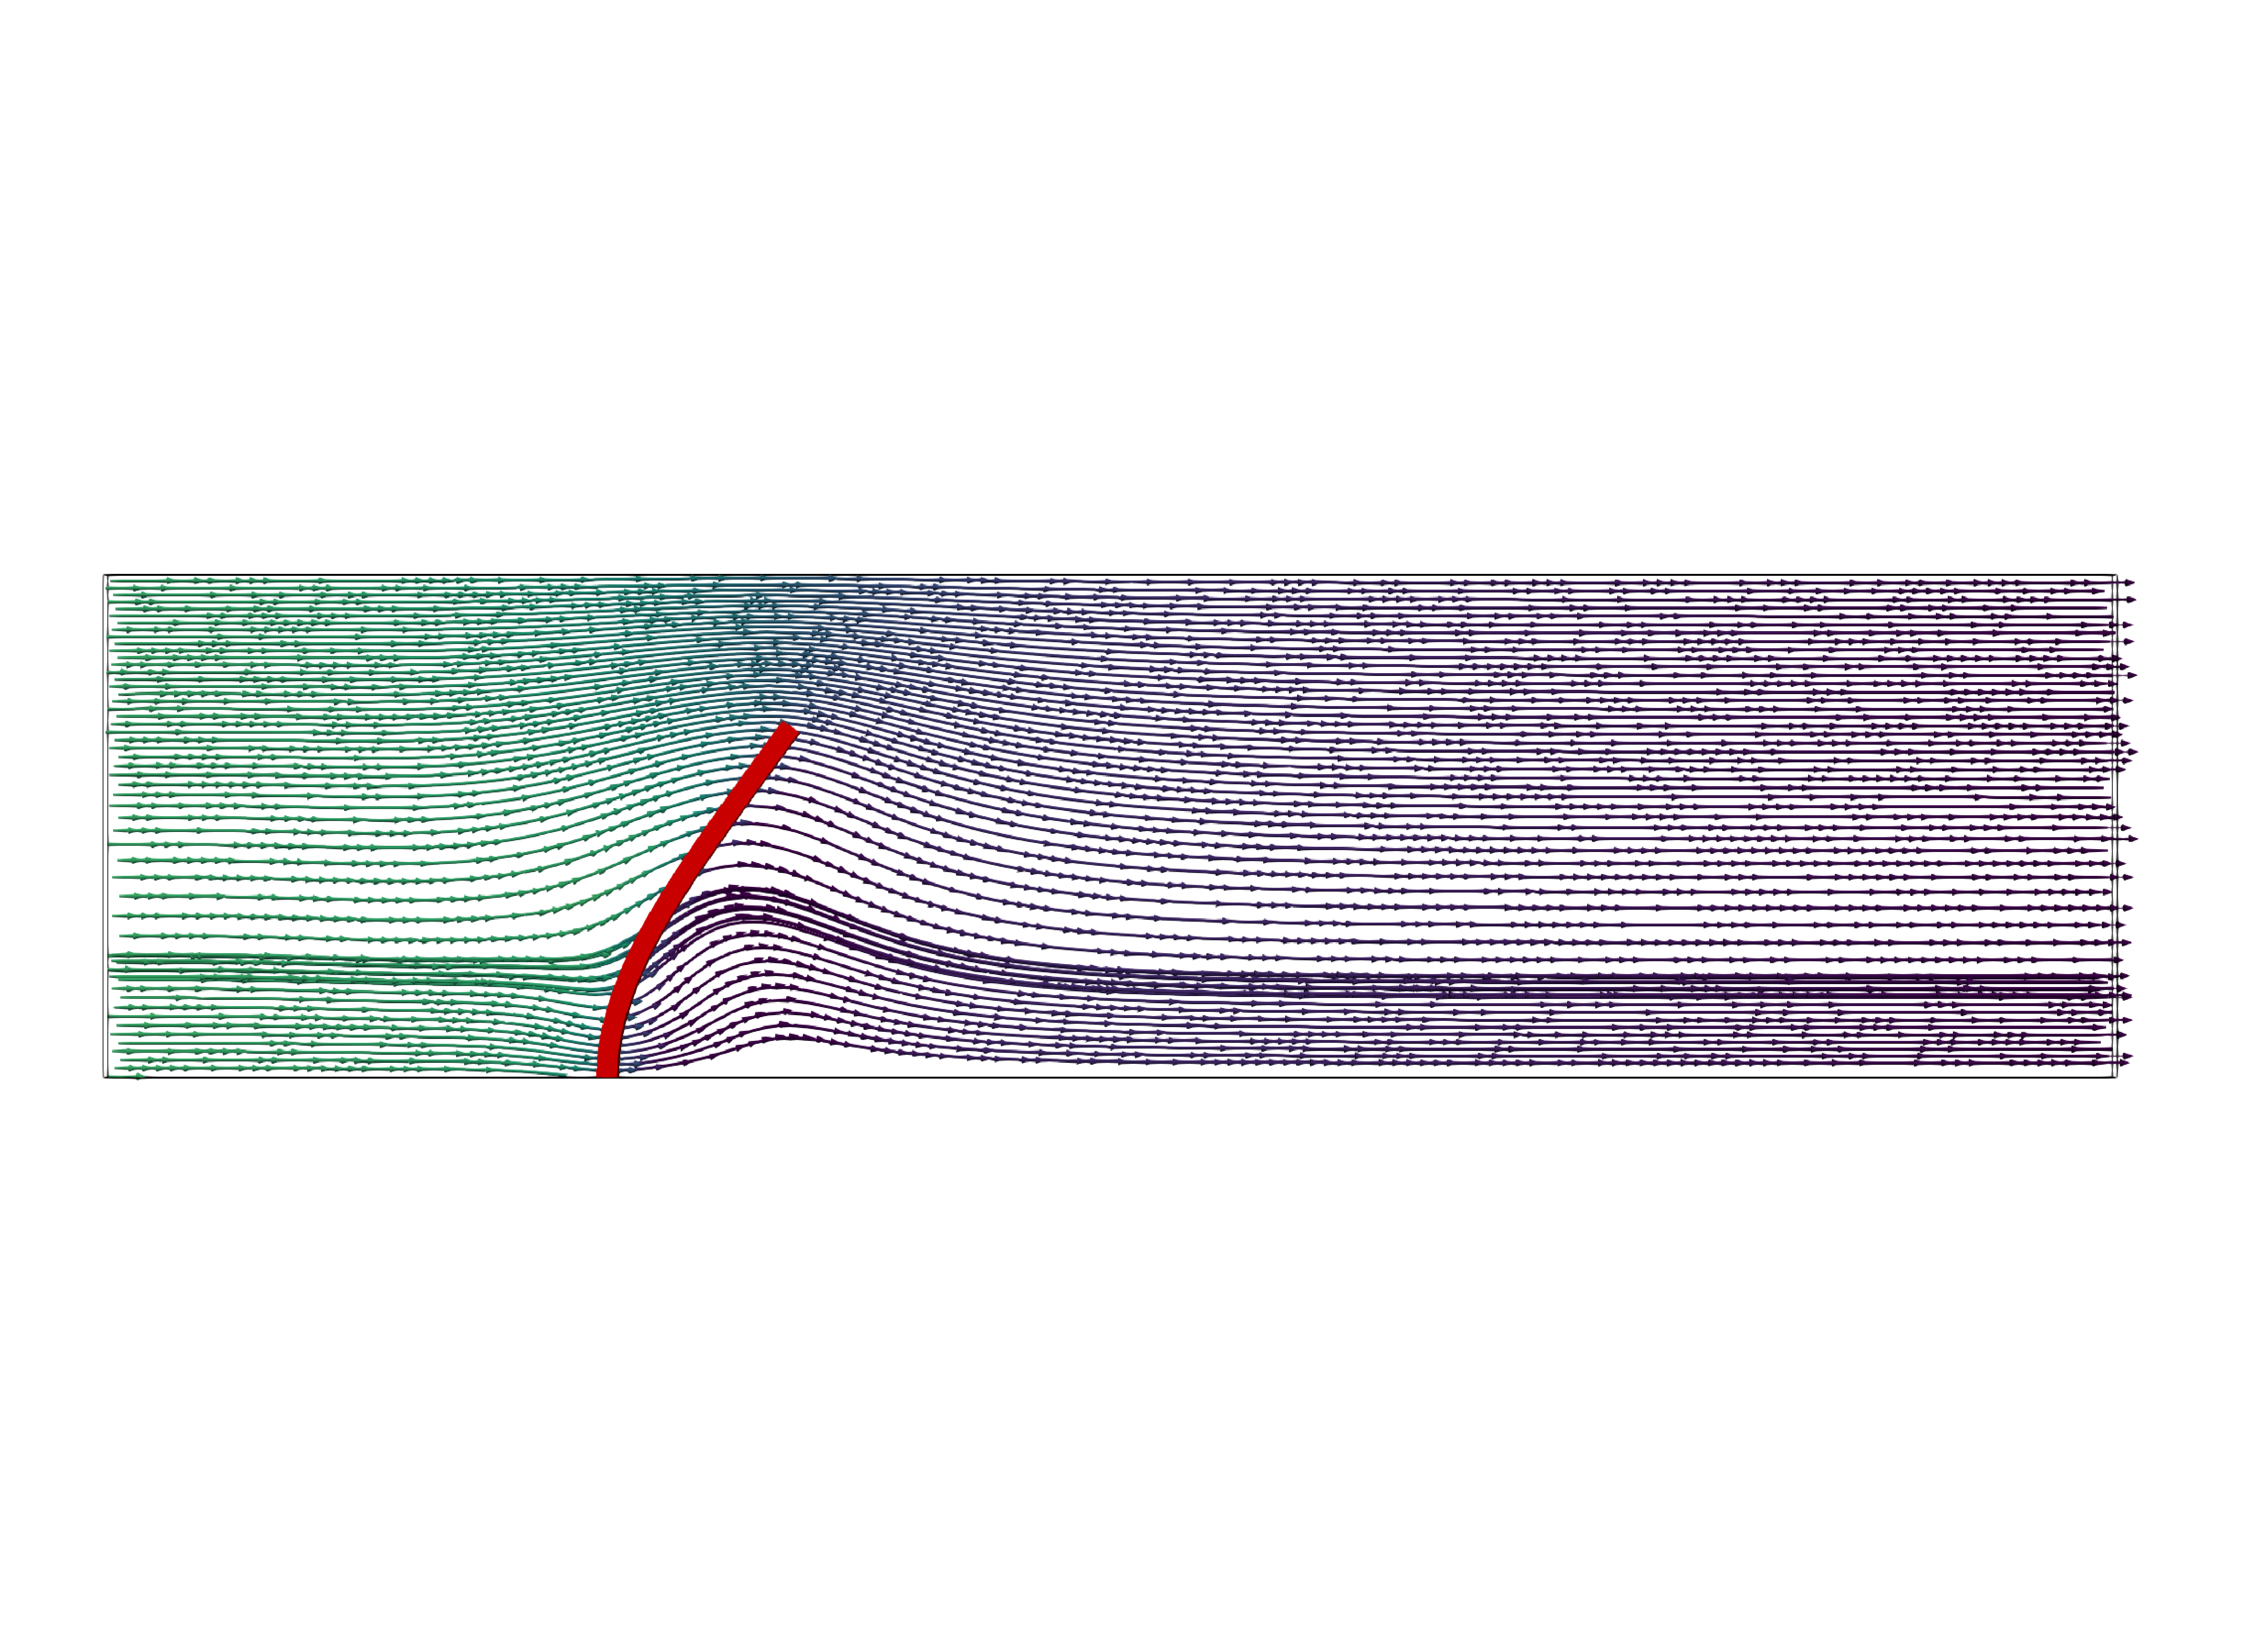
\includegraphics[width=\linewidth,trim={0 270 0 20},clip]{beamInTunnel_snapshot_t0p3.pdf}
  \caption{$t = 0.3~\mathrm{s}$}
\end{subfigure}\\[0.6em]
\begin{subfigure}[b]{0.90\textwidth}
  \centering
  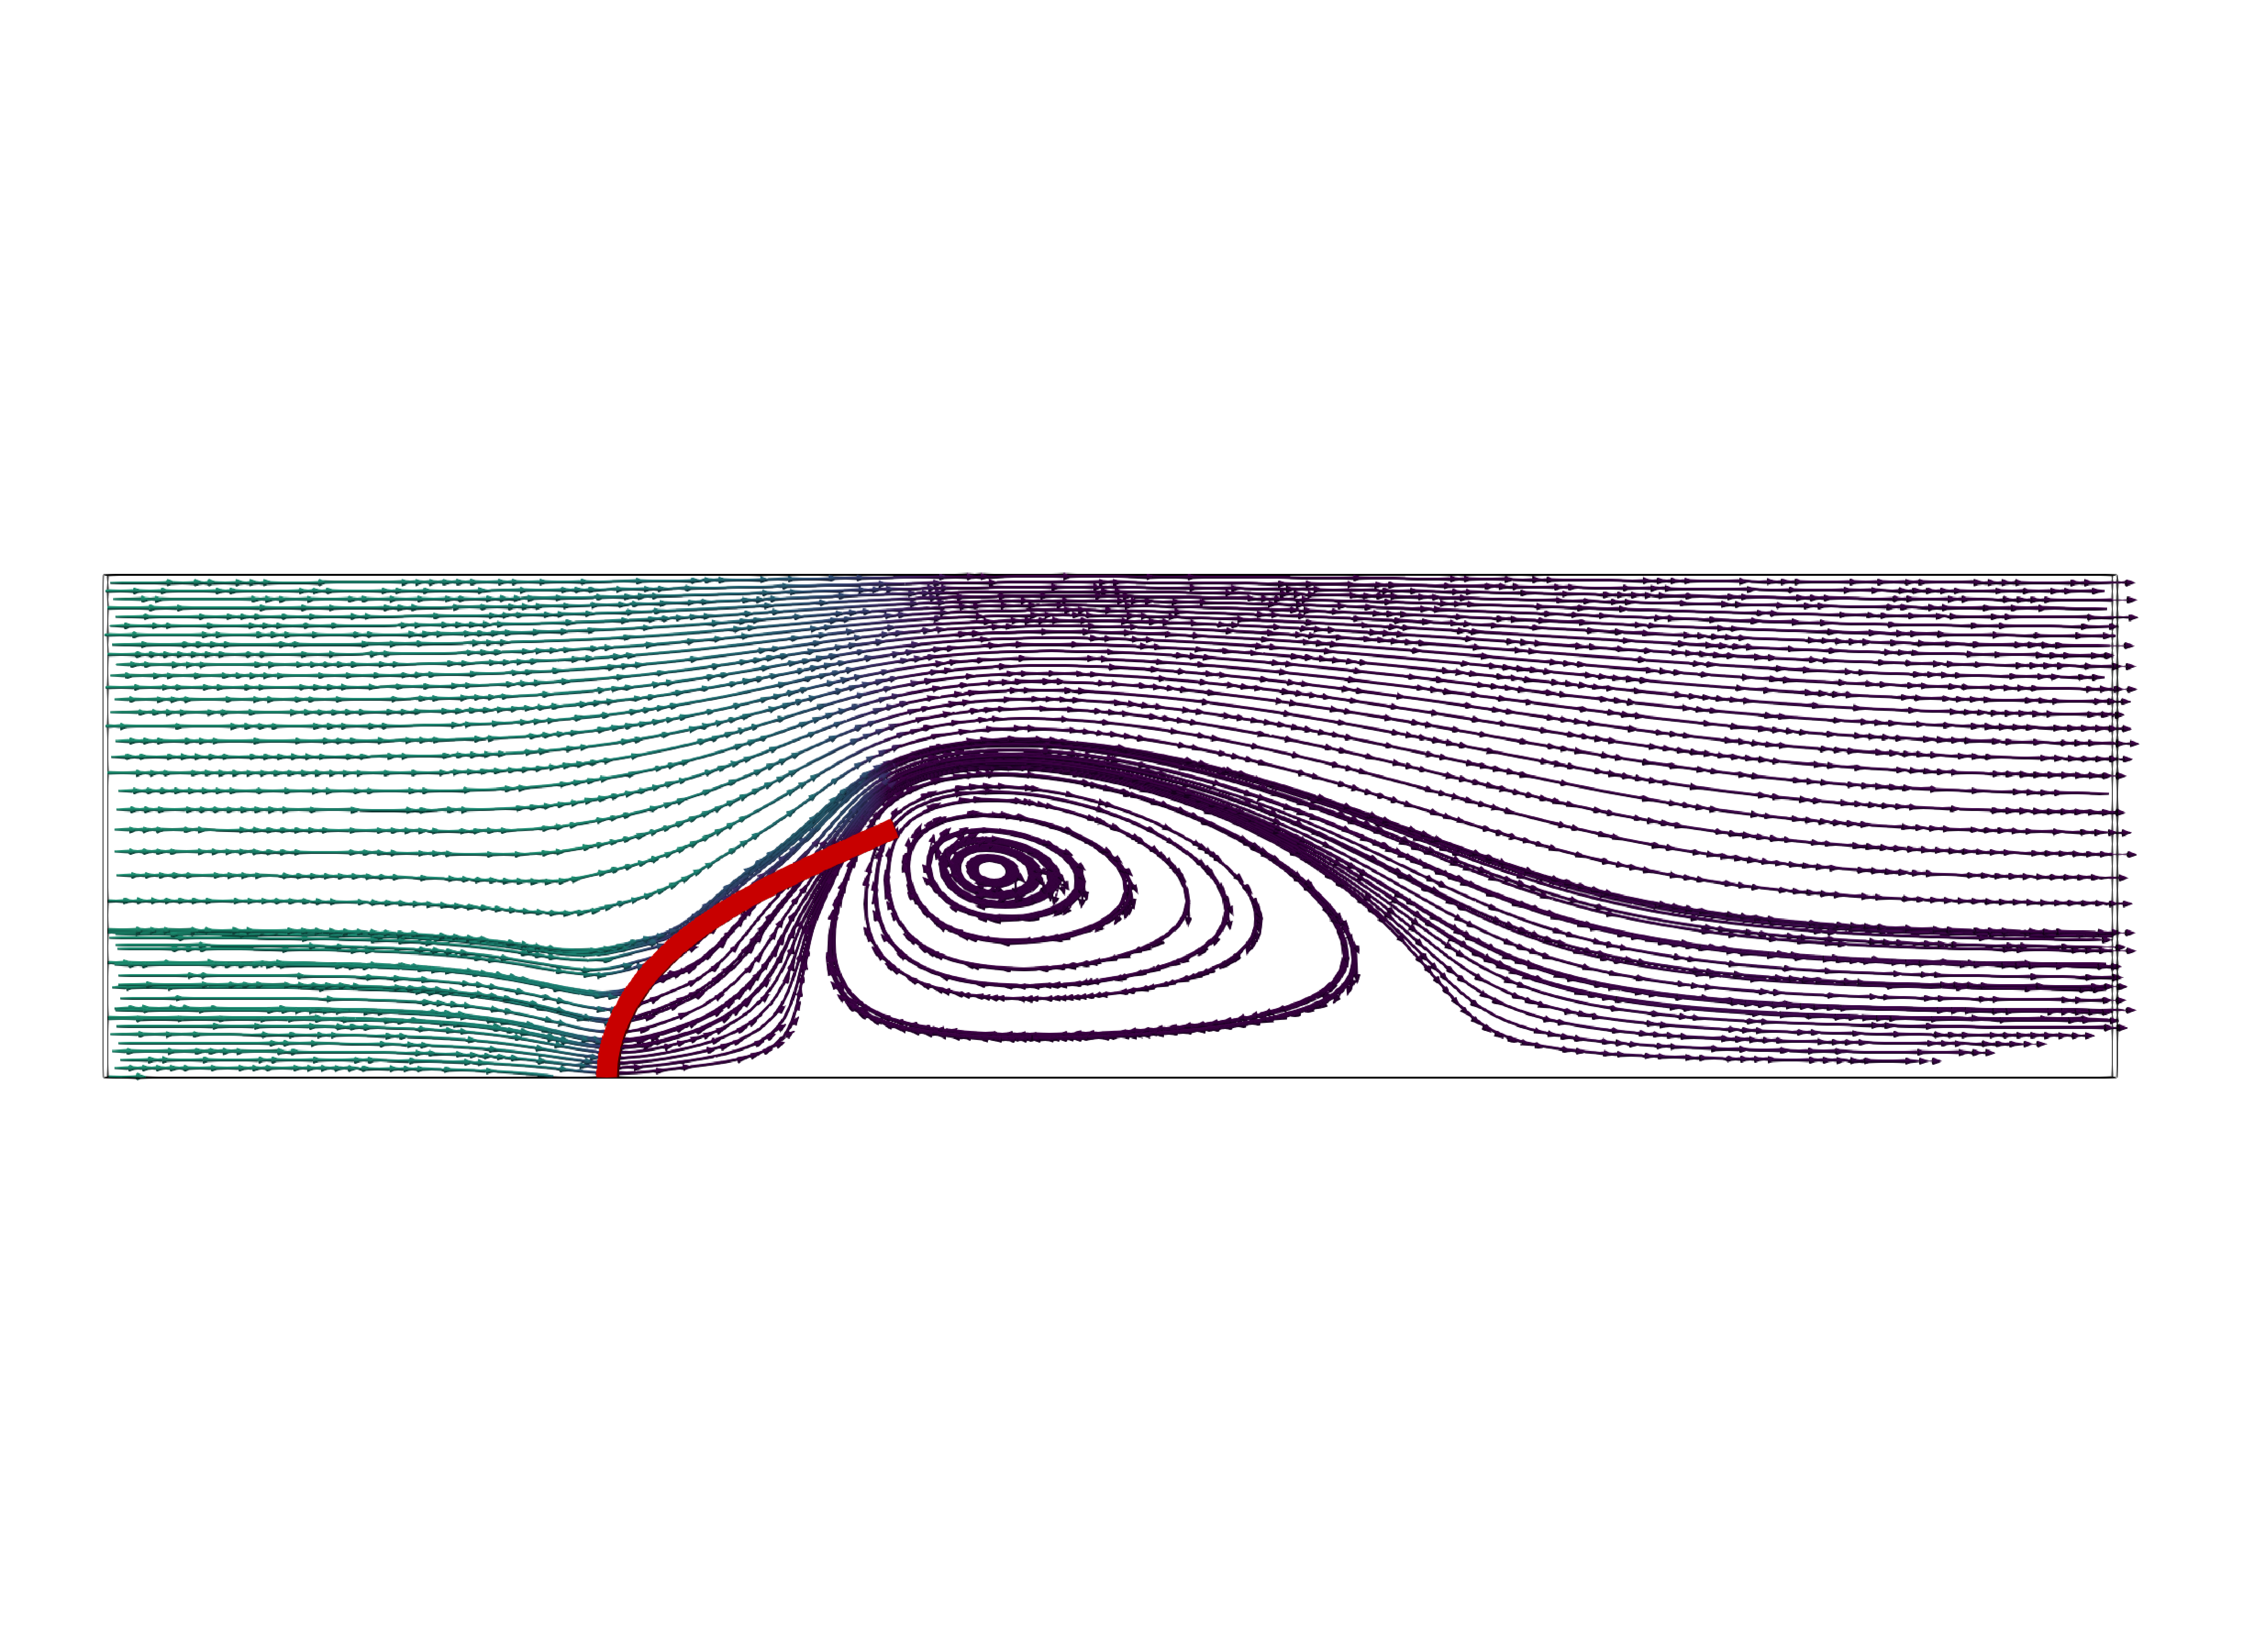
\includegraphics[width=\linewidth,trim={0 270 0 20},clip]{beamInTunnel_snapshot_t1p5.pdf}
  \caption{$t = 1.5~\mathrm{s}$}
\end{subfigure}
\caption{Flow field during the early transient and at the steady asymptote. Streamlines are coloured by velocity magnitude (in $\mathrm{m\,s^{-1}}$, common scale) and the deflected cantilever is rendered in red. At $t = 0.3~\mathrm{s}$ the leeward recirculation cell has not yet formed; at $t = 1.5~\mathrm{s}$ the accelerated jet between the bent tip and the upper symmetry boundary and the leeward eddy are both fully developed.}
\label{fig:beamInTunnel_snapshots}
\end{figure}

This picture is consistent with the mechanism that underlies the steady balance. As the cantilever deflects, it forces the incoming flow into the narrowing upper portion of the channel, raising the local velocity above the tip and therefore the drag transferred to the beam, until the elastic restoring moment matches it. The same flow features are those captured by the steady-CFD calibration on the equivalent rigid plate, which justifies transferring $C_{dn}$ into the coupled run. The stagnation region and the accelerated jet also explain why the steady tip displacement is sensitive to the upstream sampling distance. The sample must be taken beyond the stagnation region, which sets the lower end of the admissible range of $r_s$, and short of both the jet and the inlet plane, which set the upper end.

\subsection{Numerical sensitivity studies}
\label{sec:beamtunnel_sensitivity}

Six sensitivity studies establish the converged status of the result. Each perturbs a single parameter around a baseline of $150 \times 38$ fluid cells, $N_b = 20$ beam cells, $\Delta t = 10^{-4}~\mathrm{s}$, $\varepsilon = 6\times10^{-4}~\mathrm{m}$, $r_s = 3.18~\mathrm{mm}$, and the baseline solver tolerance set.

\paragraph{Fluid mesh, beam mesh, and time step.}
Figure~\ref{fig:beamInTunnel_discretisation} collects the three discretisation studies. Five fluid meshes are compared, each successive mesh halving the cell size in both directions, from ultra-coarse ($19 \times 5$) up to fine ($300 \times 76$). The coarse, base, and fine meshes give $5.699$, $5.725$ and $5.728~\mathrm{mm}$, within $0.5\%$ of one another, and the corresponding trajectories are visually indistinguishable. Only the two coarsest meshes are under-resolved, the extra-coarse mesh giving $5.701~\mathrm{mm}$ with only ten cells across the channel and the ultra-coarse mesh $5.800~\mathrm{mm}$, where the additional offset reflects an inability to resolve the velocity gradient between the deflected beam and the upper boundary. This insensitivity is consistent with the regularised-source nature of the forcing, since the beam force is smeared over several fluid cells rather than acting on a no-slip interface, so the velocity field does not develop the sharp boundary-layer profile that would require fine wall-normal grading.

Four beam discretisations spanning $N_b = 20$ to $160$ give $5.71$, $5.73$, $5.73$, and $5.72~\mathrm{mm}$, within $0.3\%$ of one another and visually indistinguishable throughout. Three effects act in the same direction here. The deformed shape is close to the first bending mode and carries no sharp curvature, so a handful of points already capture it; the extent of the fluid momentum source is set by the kernel width rather than by the beam cell spacing, so once the beam discretisation is finer than the kernel the extra cells only redistribute the same total force across overlapping kernels; and the closure samples the upstream velocity once per beam cell, so once adjacent sampling points fall within a single fluid cell the refinement repeats the same sampled value. The coarsest discretisation is therefore adopted as the baseline.

The time step is varied over a factor of $500$, from $2\times10^{-2}$ down to $4\times10^{-5}~\mathrm{s}$, and across the entire stable range the steady plateau is recovered within $\pm 0.1\%$ of $5.725~\mathrm{mm}$, the transient shape differing only slightly during the build-up. The response is monotonic with a single slow timescale, so even a coarse temporal discretisation captures the asymptotic equilibrium, and steps larger than $2\times10^{-2}~\mathrm{s}$ trigger instability in the partitioned coupling. The base step of $10^{-4}~\mathrm{s}$ is therefore chosen not to converge the steady displacement, which would tolerate a much larger step, but to resolve the early transient accurately enough for the trace in Figure~\ref{fig:beamInTunnel_verification} to be comparable with the reference solutions.

\begin{figure}[!ht]
\centering
\begin{subfigure}[b]{0.32\textwidth}
  \centering
  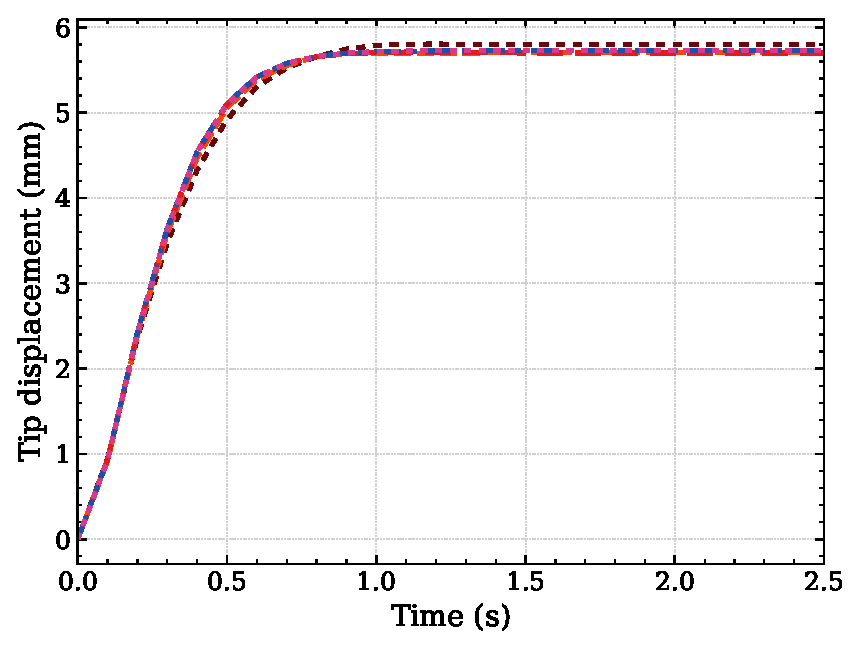
\includegraphics[width=\linewidth]{mesh_study.pdf}
  \caption{fluid mesh}
\end{subfigure}\hfill
\begin{subfigure}[b]{0.32\textwidth}
  \centering
  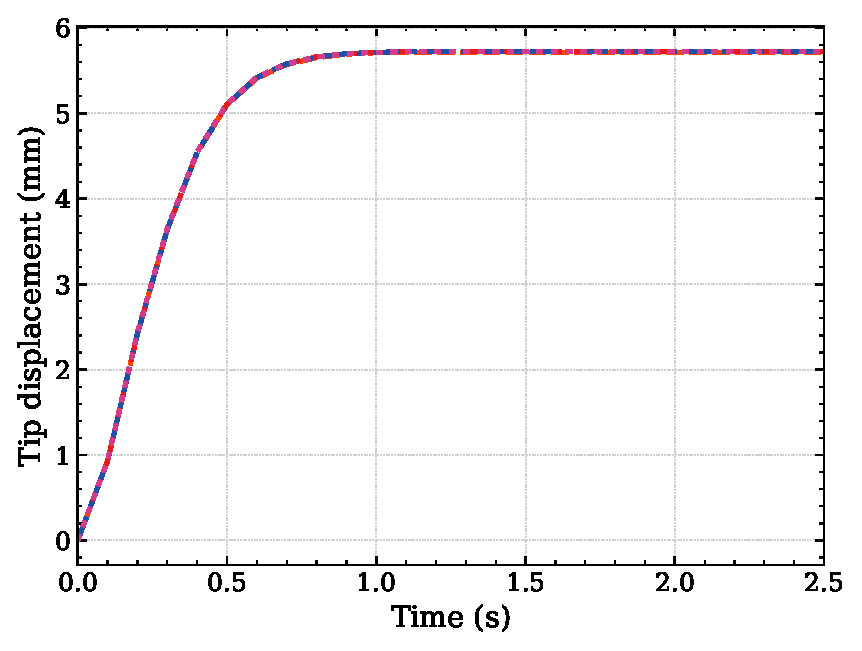
\includegraphics[width=\linewidth]{bms_study.pdf}
  \caption{beam mesh}
\end{subfigure}\hfill
\begin{subfigure}[b]{0.32\textwidth}
  \centering
  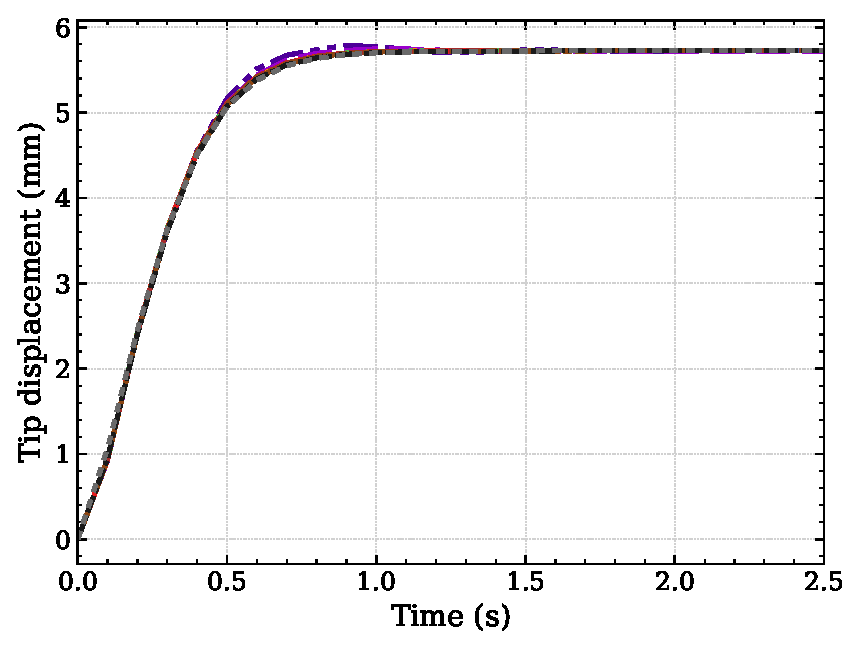
\includegraphics[width=\linewidth]{dt_study.pdf}
  \caption{time step}
\end{subfigure}\\[0.6em]
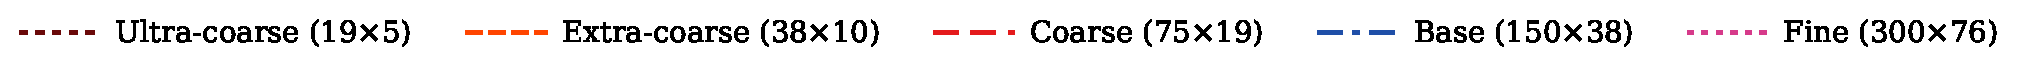
\includegraphics[width=\textwidth]{mesh_studyLegend.pdf}\\[0.2em]
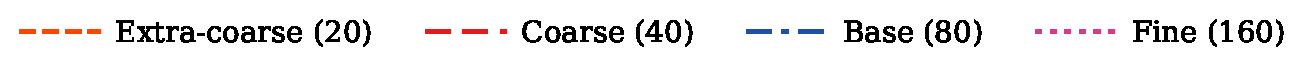
\includegraphics[width=\textwidth]{bms_studyLegend.pdf}\\[0.2em]
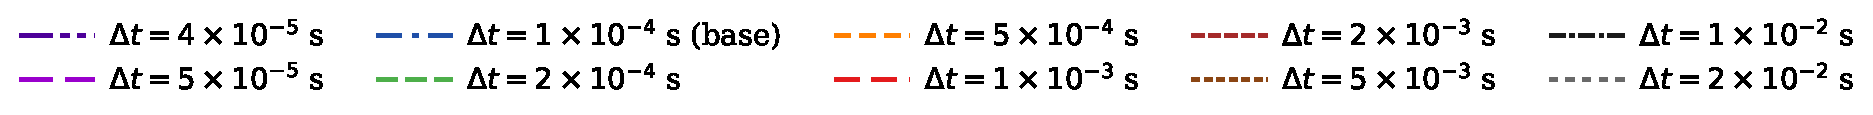
\includegraphics[width=\textwidth]{dt_studyLegend.pdf}
\caption{Discretisation studies for the flexible-beam-in-channel problem, showing the transient tip horizontal displacement for (a) five successively refined fluid meshes, (b) four beam discretisations spanning $N_b = 20$ to $160$ cells, and (c) time steps spanning a factor of $500$. Legends for the three studies are stacked below the panels in the same order. Within each study the converged traces are visually indistinguishable in the steady regime.}
\label{fig:beamInTunnel_discretisation}
\end{figure}

\paragraph{Regularisation kernel width.}
Figure~\ref{fig:beamInTunnel_operator}(a) examines the sensitivity to the Gaussian kernel width of Eq.~\eqref{eq:almGaussian}. Following the dual normalisation of \citet{bral_actuator_2025}, each value is expressed both as a multiple of the base-mesh cell size $\Delta x = 2.67\times10^{-4}~\mathrm{m}$ and of the cross-section side $a$, so the kernel can be read relative to both the discretisation and the geometric size of the structure. Because the kernel is normalised so that the total force on the fluid is independent of its width (Section~\ref{sec:almProjection}), the sensitivity measured here is only the indirect effect of the kernel on the surrounding velocity field, which modifies the upstream-sampled velocity.

Within the admissible range $1.12\,\Delta x \le \varepsilon \le 3.75\,\Delta x$, equivalently $0.75\,a$ to $2.5\,a$, the steady tip displacement varies monotonically from $5.09$ to $6.26~\mathrm{mm}$, a spread of approximately $20\%$ (Table~\ref{tab:beamtunnel_operator_cases}). Smaller $\varepsilon$ concentrates the reaction closer to the centreline, producing a more localised wake and a lower sampled velocity, hence smaller drag and smaller deflection, while larger $\varepsilon$ spreads the reaction into the freestream and raises the sampled velocity. The baseline $\varepsilon = 2.25\,\Delta x = 1.5\,a$ sits above the minimum required for a resolved projection and clear of the upper boundary, and it is the operating point at which the result lands closest to the literature range. The outlier at $5.62\,\Delta x$ corresponds to a kernel so wide that its tail overlaps the upper symmetry boundary. The mass falling outside the domain is truncated, the nodal normalisation redistributes the truncated fraction along the whole node support instead of preserving the local profile, and the momentum injected near the beam therefore drops, which is why its displacement of $5.53~\mathrm{mm}$ falls back below the monotonic trend. The increasing relation between $\varepsilon$ and tip displacement holds only while the kernel stays clear of the walls.

\paragraph{Upstream sampling distance.}
Figure~\ref{fig:beamInTunnel_operator}(b) reports the sensitivity to the offset $r_s$. In an unbounded flow this offset is chosen large enough to sample the undisturbed freestream rather than the stagnation-affected velocity adjacent to the beam, but in a confined channel it must also remain inside the domain and below the upper symmetry plane. Over the admissible range the steady displacement varies monotonically from $4.44~\mathrm{mm}$ at $r_s = 0.53~\mathrm{mm}$ to $6.20~\mathrm{mm}$ at $4.77~\mathrm{mm}$, a spread of approximately $31\%$. The smallest offset samples within the beam's own stagnation zone and the largest samples the accelerated jet between the deflected beam and the upper boundary. The case $r_s = 6.36~\mathrm{mm}$ pushes the sampling point upstream of the inlet for the lower part of the beam and lies outside the admissible range.

\begin{figure}[!ht]
\centering
\begin{subfigure}[b]{0.48\textwidth}
  \centering
  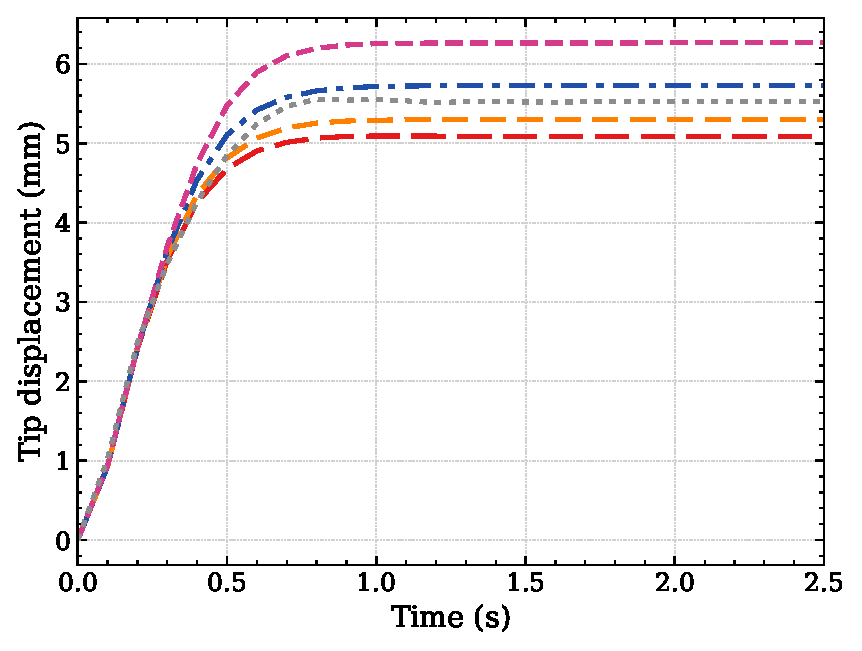
\includegraphics[width=\linewidth]{eps_study.pdf}
  \caption{kernel width $\varepsilon$}
\end{subfigure}\hfill
\begin{subfigure}[b]{0.48\textwidth}
  \centering
  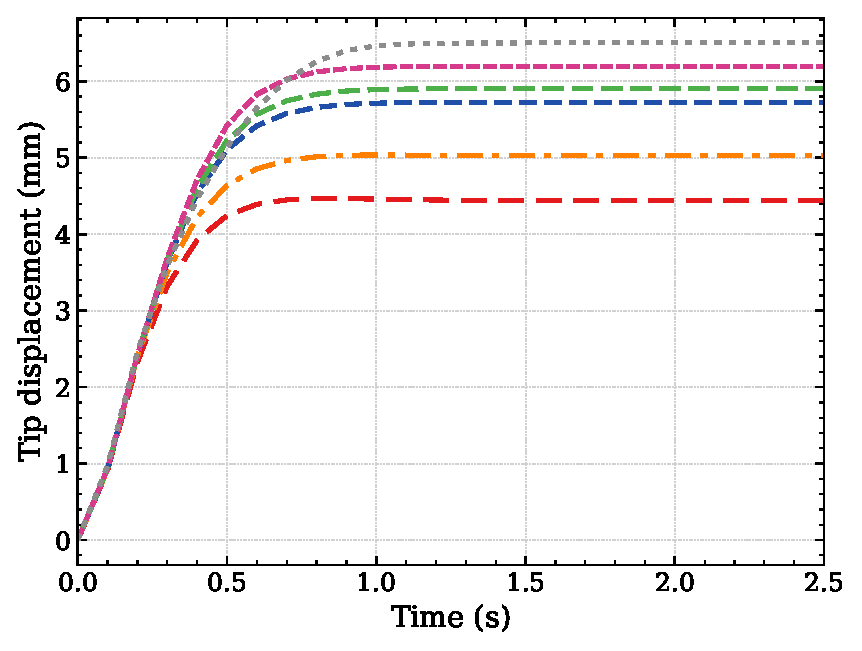
\includegraphics[width=\linewidth]{sampling_study.pdf}
  \caption{sampling offset $r_s$}
\end{subfigure}\\[0.6em]
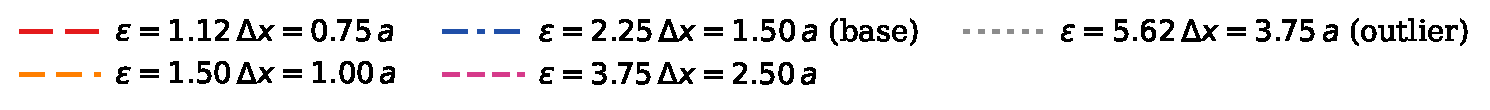
\includegraphics[width=\textwidth]{eps_studyLegend.pdf}\\[0.2em]
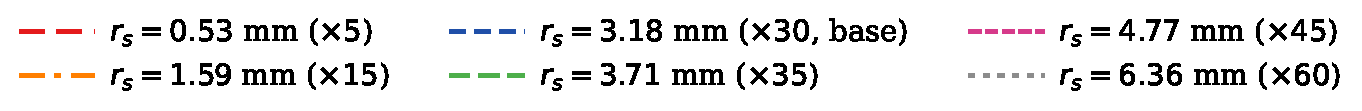
\includegraphics[width=\textwidth]{sampling_studyLegend.pdf}
\caption{Sensitivity of the steady tip displacement to the two coupling-operator settings. (a) Gaussian kernel width, each case labelled both in units of the base-mesh cell size $\Delta x = 2.67\times10^{-4}~\mathrm{m}$ and the cross-section side $a$; the case $\varepsilon = 5.62\,\Delta x$ overlaps the upper symmetry boundary and is excluded. (b) Upstream sampling offset; the smallest sample lies in the stagnation zone and the largest beyond the inlet, both shown in grey. Legends for the two studies are stacked below the panels in the same order, and the individual values are listed in Table~\ref{tab:beamtunnel_operator_cases}. Unlike the discretisation studies of Figure~\ref{fig:beamInTunnel_discretisation}, both parameters change the response by tens of percent.}
\label{fig:beamInTunnel_operator}
\end{figure}

\begin{table}[!ht]
\centering
\small
\caption{Kernel-width and sampling-distance studies. Steady tip displacement for each Gaussian regularisation width $\varepsilon$, listed as a multiple of the base-mesh cell size $\Delta x = 2.67\times10^{-4}~\mathrm{m}$ and of the cross-section side $a = 4\times10^{-4}~\mathrm{m}$, and for each upstream sampling offset $r_s$.}
\label{tab:beamtunnel_operator_cases}
\setlength{\tabcolsep}{6pt}
\renewcommand{\arraystretch}{1.15}
\begin{tabular}{c c c c l @{\qquad} c c l}
\toprule
\multicolumn{5}{l}{\textbf{Kernel width}} & \multicolumn{3}{l}{\textbf{Sampling offset}} \\
$\varepsilon$ (m) & $\varepsilon/\Delta x$ & $\varepsilon/a$ & Tip (mm) & Note & $r_s$ (mm) & Tip (mm) & Note \\
\midrule
$3.0\times10^{-4}$ & $1.12$ & $0.75$ & $5.09$ & lower bound        & $0.53$ & $4.44$ & stagnation zone \\
$4.0\times10^{-4}$ & $1.50$ & $1.00$ & $5.30$ &                    & $1.59$ & $5.03$ & \\
$6.0\times10^{-4}$ & $2.25$ & $1.50$ & $5.73$ & baseline           & $3.18$ & $5.73$ & baseline \\
$1.0\times10^{-3}$ & $3.75$ & $2.50$ & $6.26$ & upper bound        & $3.71$ & $5.90$ & \\
$1.5\times10^{-3}$ & $5.62$ & $3.75$ & $5.53$ & overlaps top wall  & $4.77$ & $6.20$ & upper bound \\
                   &        &        &        &                    & $6.36$ & $6.50$ & upstream of inlet \\
\bottomrule
\end{tabular}
\end{table}

The baseline $r_s = 3.18~\mathrm{mm}$ lands in the middle of the admissible range and yields, together with the kernel-width baseline, the result closest to the literature range. Both settings therefore function as effective calibration parameters rather than discretisation-only convergence controls, and in this confined channel they act together as a calibration of the quasi-steady closure to the local blockage. This affects how the benchmark outcome should be described. Only $C_{dn}$ was fixed independently of the reference; the pair $(\varepsilon, r_s)$ was selected within its admissible plateau with the reference result in view, so the agreement is an assessment against other numerical solutions with two calibrated operator settings, not a fully blind prediction. The selected pair is carried \emph{unchanged} into the benchmark of Section~\ref{sec:leaflet}, where it faces four forcing conditions on which it was not selected, and the wave-flume case of Section~\ref{sec:flexveg} sizes the kernel by the same rule relative to the local cell size. What those later cases test is the transferred settings, not the settings themselves.

\paragraph{Solver tolerance hierarchy.}
The remaining numerical artefact is the iterative tolerance of the structural Newton solver and the PIMPLE outer loop. Table~\ref{tab:beamtunnel_tol_cases} reports three successively tightened configurations. The loose-structural configuration over-predicts the steady displacement by $3.3\%$ and drifts slowly away from a transient overshoot, which is the characteristic signature of a partitioned coupling whose structural side has not converged within each time step. Tightening the Newton tolerance alone reduces both the overshoot and the drift to under $1\%$, and increasing the PIMPLE outer-iteration count on top brings the plateau within $0.1\%$ of its asymptotic value. That third configuration is used for Figure~\ref{fig:beamInTunnel_verification} and for all the studies above. The hierarchy separates two contributions. Tightening the Newton tolerance removes the bulk of the error at negligible cost, because the structural solve is cheap relative to the fluid solve, whereas raising the outer-iteration count from one to twenty closes the remaining sub-percent error but multiplies the per-step fluid cost by roughly five to ten. The dominant iterative error is therefore on the structural side. The last step also bounds the error introduced by freezing the interface force for the duration of the time step (Section~\ref{sec:almParallelSearch}), because driving the pressure--velocity system to convergence against that frozen force changes the answer by $0.1\%$.

\begin{table}[!ht]
\centering
\small
\caption{Solver-tolerance hierarchy. The structural Newton tolerance and the number of PIMPLE outer iterations $n_{\mathrm{out}}$ are tightened in turn. The last configuration is adopted for the verification figure and all sensitivity studies.}
\label{tab:beamtunnel_tol_cases}
\setlength{\tabcolsep}{5pt}
\renewcommand{\arraystretch}{1.15}
\begin{tabular}{l c c c l}
\toprule
Configuration & Newton tol. & $n_{\mathrm{out}}$ & Tip (mm) & Note \\
\midrule
Loose structural          & $10^{-6}$ & $1$  & $5.92$ & overshoot, slow drift \\
Tight structural          & $10^{-9}$ & $1$  & $5.75$ & drift below $1\%$ \\
Tight structural + PIMPLE & $10^{-9}$ & $20$ & $5.73$ & reference (within $0.1\%$) \\
\bottomrule
\end{tabular}
\end{table}

Taken together, the six studies confirm that the steady tip displacement of $5.73~\mathrm{mm}$ is converged in the discretisation sense. It stays inside the literature band of $4.7$ to $6.0~\mathrm{mm}$, and where it sits within that band comes from reducing the two-dimensional structure to a one-dimensional beam loaded by a distributed normal drag. This verifies the coupling against reference solutions obtained with other methods for steady, viscous-dominated flow in a confined channel, which is a check against other numerical solutions rather than a validation against physical measurements, and it motivates moving to the time-periodic benchmark of the next section.
